\documentclass[aspectratio=169]{beamer}
\usepackage[utf8]{inputenc}
\usepackage[T1]{fontenc}
\usepackage[brazil]{babel}
\usepackage{ragged2e}
\usepackage{booktabs}
\usepackage{verbatim}
\usetheme{AnnArbor}
\usecolortheme{orchid}
\usefonttheme[onlymath]{serif}
\usepackage{listings}
\usepackage{colortbl}
\usepackage{array}

\newcolumntype{C}[0]{>{\centering\arraybackslash}p{0.4cm}}

\lstset{language=C++,
	backgroundcolor=\color{green!10},
	basicstyle=\ttfamily,
	keywordstyle=\color{blue}\ttfamily,
	stringstyle=\color{red}\ttfamily,
	commentstyle=\color{green}\ttfamily,
	morecomment=[l][\color{magenta}]{\#},
	literate=
	{á}{{\'a}}1
	{à}{{\`a}}1
	{ã}{{\~a}}1
	{â}{{\^a}}1
	{é}{{\'e}}1
	{ê}{{\^e}}1
	{í}{{\'i}}1
	{ó}{{\'o}}1
	{õ}{{\~o}}1
	{ú}{{\'u}}1
	{ü}{{\"u}}1
	{ç}{{\c{c}}}1
	{Á}{{\'A}}1
	{À}{{\`A}}1
	{Ã}{{\~A}}1
	{Â}{{\^A}}1
	{É}{{\'E}}1
	{Ê}{{\^E}}1
	{Í}{{\'I}}1
	{Ó}{{\'O}}1
	{Õ}{{\~O}}1
	{Ú}{{\'U}}1
	{Ü}{{\"U}}1
	{Ç}{{\c{C}}}1
}

\AtBeginSection[]{
  \begin{frame}
  \vfill
  \centering
  \begin{beamercolorbox}[sep=8pt,center,shadow=true,rounded=true]{title}
    \usebeamerfont{title}\insertsectionhead\par%
  \end{beamercolorbox}
  \vfill
  \end{frame}
}

\title[\sc{Estruturas Lineares}]{Estruturas Lineares}
\author[Roland Teodorowitsch]{Roland Teodorowitsch}
\institute[ALEST I - EP - PUCRS]{Algoritmos e Estruturas de Dados I - Escola Politécnica - PUCRS}
\date{4 de setembro de 2023}

\begin{document}

\justifying

%-------------------------------------------------------
\begin{frame}
	\titlepage
\end{frame}

%=======================================================
\section{Introdução}

%-------------------------------------------------------
\begin{frame}\frametitle{Leitura(s) Recomendada(s)}

\begin{columns}[T]
\begin{column}{0.15\linewidth}
\vspace{-3mm}
\begin{figure}[h]
	\centering
	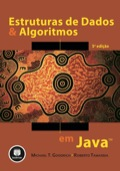
\includegraphics[height=0.3\paperheight]{imagens/livro_goodrich.jpg}
\end{figure}
\end{column}
%\vspace{3mm}
\begin{column}{0.85\linewidth}
\tiny{\textbf{Seções 3.2 (Listas simplesmente encadeadas), 3.3 (Listas duplamente encadeadas), 6.1 (Listas arranjo), 6.2 (Listas de nodos), 6,4 (Os TADs de lista e o \emph{framework} de coleções)}\\
~}\\
\scriptsize{GOODRICH, Michael T.; TAMASSIA, Roberto. \textbf{Estruturas de dados e algoritmos em Java}. Tradução: Bernardo Copstein. 5. ed. Porto Alegre: Bookman, 2013. xxii, 713 p. E-book. ISBN 9788582600191. Tradução de: Data Structures and Algorithms in Java, 5th Edition. Disponível em: \textless{}\url{https://integrada.minhabiblioteca.com.br/\#/books/9788582600191/}\textgreater{}. Acesso em: 01 ago. 2023.}
\end{column}
\end{columns}

\end{frame}

%=======================================================
\section{Tipos Abstratos de Dados}

%-------------------------------------------------------
\begin{frame}\frametitle{Abordagem OO}
\begin{itemize}
	\item Princípios da abordagem OO
	\begin{itemize}
		\item \textbf{Abstração}: representação de um objeto do mundo real, ``abstraindo-se'' os detalhes desnecessários, de forma que o objeto possa ser utilizado sem se preocupar com como ele foi implementado
		\item \textbf{Encapsulamento}: detalhes da implementação ficam escondidos e a manipulação dos dados acontede através de uma interface pública
		\item \textbf{Modularidade}: vários componentes que interagem
	\end{itemize}
	\item Abstração, Encapsulamento, Herança e Polimorfismo são considerados os 4 pilares da POO
\end{itemize}
\end{frame}

%-------------------------------------------------------
\begin{frame}\frametitle{Tipos Abstratos de Dados}
\begin{itemize}
	\item A aplicação de abstração ao projeto de estruturas de dados nos leva a \textbf{Tipos Abstratos de Dados (TAD)}
	\item TAD
	\begin{itemize}
		\item É uma especificação de um conjunto de dados e operações que podem ser executadas sobre esses dados
		\item Modelo matemático de estruturas de dados que especifica
		\begin{itemize}
			\item O tipo dos dados armazenados
			\item As operações definidas sobre esses dados
			\item Os tipos dos parâmetros dessas operações
		\end{itemize}
	\end{itemize}
	\item A separação de especificação e implementação permite usar um TAD sem conhecer nada sobre a sua implementação
	\begin{itemize}
		\item Assim, um TAD pode ter mais de uma implementação
	\end{itemize}
\end{itemize}
\end{frame}

%-------------------------------------------------------
\begin{frame}\frametitle{TAD}
\begin{itemize}
	\item Usa ``encapsulamento''
	\item Princípio: esconder detalhes de representação e direcionar o acesso aos objetos abstratos por meio de operações
	\item A representação fica protegida contra qualquer tentativa de manipulá-la diretamente (só através das operações disponíveis)
	\item Define o que cada operação faz, mas não como o faz
\end{itemize}
\end{frame}

%-------------------------------------------------------
\begin{frame}\frametitle{Tipos Abstratos de Dados}
\begin{itemize}
	\item Resumindo, TAD é uma estrutura de programa que contém
	\begin{itemize}
		\item A especificação de uma estrutura de dados
		\item Um conjunto de operações que podem ser realizadas sobre os dados encapsulados
	\end{itemize}
	\item Exemplos de TADs
	\begin{itemize}
		\item Pilhas, Filas, Deques e Listas
	\end{itemize}
	\item Essas estruturas são classificadas como lineares
	\begin{itemize}
		\item Representam coleções de elementos linearmente organizados que oferecem métodos para inserir, acessar e remover elementos
		\item Tem a ordem interna de seus elementos definida pela forma como são feitas inserções e remoções na estrutura
		\item Costuma ter duas extremidades (esquerda e direita; frente e traseira; cabeça e cauda; ...)
	\end{itemize}
\end{itemize}
\end{frame}

%-------------------------------------------------------
\begin{frame}\frametitle{Estruturas Lineares}
\begin{itemize}
	\item \textbf{Lista}
	\begin{itemize}
		\item Organiza os dados de maneira sequencial (não necessariamente de forma física, mas sempre existe uma ordem lógica entre os elementos)
		\item Permite inserção, acesso e remoção de elementos
	\end{itemize}
	\item \textbf{Pilha}
	\begin{itemize}
		\item Usa a política \emph{LIFO -- Last In First Out} (o último elemento que entrou, é o primeiro a sair)
		\item Possui apenas uma entrada, chamada de topo, a partir da qual os dados entram e saem dela
	\end{itemize}
	\item \textbf{Fila}
	\begin{itemize}
		\item Usa a política \emph{FIFO -- First In First Out} (o primeiro elemento a entrar será o primeiro a sair)
		\item Os elementos entram por um lado (``cauda'' ou parte de trás) e saem por outro (``cabeça'' ou parte da frente)
	\end{itemize}
	\item \textbf{Deque} (\emph{Double-Ended QUEue})
	\begin{itemize}
		\item Os elementos entram e saem por qualquer uma das extremidades (cauda ou cabeça) da lista
	\end{itemize}
\end{itemize}
\end{frame}

%-------------------------------------------------------
\begin{frame}\frametitle{Estruturas Lineares}
\begin{itemize}
	\item Permitem representar um conjunto de dados de um mesmo tipo (com alguma afinidade) de forma a preservar a relação de ordem entre seus elementos
	\item Cada elemento da estrutura é chamado de nó, ou nodo.
	\item Uma estrutura linear é definida como:
	\begin{itemize}
		\item Um conjunto de $N$ nós, organizados de forma a refletir a posição relativa dos mesmos
		\item Se $N > 0$, os nós da estrutura serão $x_1$, $x_2$, ..., $x_N$, 
		\begin{itemize}
			\item $x_1$ é o primeiro nó
			\item Para $1 < k < N$, o nó $x_k$ é precedido pelo nó $x_{k-1}$ e seguido pelo nó $x_{k+1}$
			\item $x_N$ é o último nó
		\end{itemize}
		\item Quando $N = 0$, diz-se que a estrutura está vazia
	\end{itemize}
\end{itemize}
\end{frame}

%-------------------------------------------------------
\begin{frame}\frametitle{Exemplos de Estruturas Lineares}
\begin{itemize}
	\item Pessoas na fila de um caixa (ordem definida pela chegada e posição na fila)
	\item Pessoas na sala de espera de um consultório (ordem definida pela chegada)
	\item Conjunto de notas dos alunos de uma turma
	\item Itens no estoque de uma loja
	\item Palavras de um texto
	\item Letras de uma palavra
	\item Especificação de operações e operandos em uma expressão matemática
	\item Dias da semana
	\item Relação de compromissos
	\item Pilha de livros
	\item Cartas de um baralho
	\item etc.
\end{itemize}
\end{frame}

%-------------------------------------------------------
\begin{frame}[fragile]\frametitle{Alocação de Estruturas Lineares}
\begin{itemize}
	\item Estruturas lineares podem ser alocadas de forma:
	\begin{itemize}
		\item \textbf{Sequencial ou Contígua}\\Os nós, além de estarem em uma sequência lógica, também estão \textbf{fisicamente em sequência}
\begin{figure}[h]
	\centering
	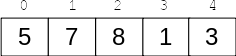
\includegraphics[height=0.10\paperheight]{imagens/vetor.png}
\end{figure}
		\item \textbf{Encadeada}\\Os nós são alocados dinamicamente e são ligados entre si, de forma que há uma sequência lógica, mas fisicamente os nós NÃO precisam estar contíguos
\begin{figure}[h]
	\centering
	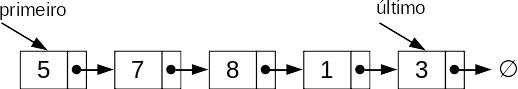
\includegraphics[height=0.15\paperheight]{imagens/lista_simplesmente_encadeada.png}
\end{figure}
	\end{itemize}
	\item Cada forma tem as suas vantagens e desvantagens
\end{itemize}
\end{frame}

%-------------------------------------------------------
\begin{frame}\frametitle{Alocação Sequencial ou Contígua de Estruturas Lineares}
\begin{itemize}
	\item Nós adjacentes na estrutura são armazenados em endereços contíguos na memória física e o tamanho da estrutura é fixo
	\item A implementação é feita com vetores (arranjos ou \emph{arrays}), que podem ser alocados de forma estática ou dinâmica
	\item Pode-se trabalhar com vetores parcialmente prenchidos
	\item O acesso é rápido
	\item NÃO é possível ter espaços vazios (não utilizados) no meio da estrutura (a não ser no final, para vetores parcialmente preenchidos)
	\item Inserção e Remoção de elementos no meio exige movimentação de elementos
	\item Para estruturas alocadas dinamicamente, pode-se: alocar um novo vetor, copiar os elementos do antigo para o novo, desalocar o antigo e passar a usar o novo -- mas isto pode ser custoso
\end{itemize}
\end{frame}
	
%-------------------------------------------------------
\begin{frame}[fragile]\frametitle{Alocação Sequencial ou Contígua de Estruturas Lineares (vetores.cpp)}
\lstinputlisting[basicstyle=\ttfamily\tiny]{src/vetores.cpp}
\end{frame}

%-------------------------------------------------------
\begin{frame}[fragile]\frametitle{Alocação Sequencial ou Contígua de Estruturas Lineares (vetores2.cpp)}
\lstinputlisting[basicstyle=\ttfamily\tiny]{src/vetores2.cpp}
\end{frame}

%-------------------------------------------------------
\begin{frame}\frametitle{Alocação Encadeada de Estruturas Lineares}
\begin{itemize}
	\item Os elementos da estrutura seguem uma ordem lógica, mas \textbf{NÃO estão necessariamente armazenados sequencialmente na memória}
	\item A relação lógica de ordem é implementada através de uma ligação (referência ou armazenamento de endereço) entre os nodos
	\item Estruturas lineares encadeadas são chamadas de \textbf{listas encadeadas}, sendo que cada nodo pode armazenar uma referência para o próximo elemento (lista simplesmente encadeada)
\begin{figure}[h]
	\centering
	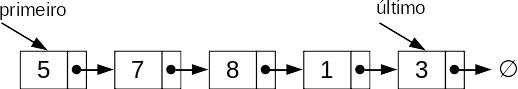
\includegraphics[height=0.15\paperheight]{imagens/lista_simplesmente_encadeada.png}
\end{figure}
	\item Ou para o elemento anterior e para o próximo elemento (lista duplamente encadeada)
\begin{figure}[h]
	\centering
	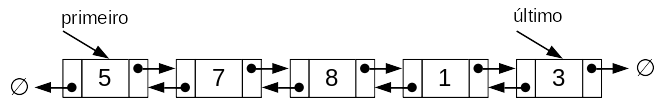
\includegraphics[height=0.16\paperheight]{imagens/lista_duplamente_encadeada.png}
\end{figure}
	\item A estrutura pode aumentar e diminuir em tempo de execução
\end{itemize}
\end{frame}

%-------------------------------------------------------
\begin{frame}\frametitle{Alocação Encadeada de Estruturas Lineares}
\begin{itemize}
	\item Quando for necessário inserir um elemento na estrutura, deve-se:
	\begin{itemize}
		\item Alocar um novo nodo
		\item Preencher as informações no nodo
		\item Inserir o novo nodo em determinada posição da estrutura (o que exige ajustes em alguns encadeamentos)
	\end{itemize}
	\item Alocação encadeada será útil quando:
	\begin{itemize}
		\item Não é possível prever o número de entradas de dados em tempo de compilação
		\item For mais fácil aplicar determinada operação sobre a estrutura encadeada
	\end{itemize}
\end{itemize}
\end{frame}

%-------------------------------------------------------
\begin{frame}\frametitle{Operações Básicas sobre Estruturas Lineares}
\begin{itemize}
	\item Criação da estrutura
	\item Destruição da estrutura
	\item Inserção de um elemento na estrutura
	\item Remoção de um elemento da estrutura
	\item Acesso a um elemento da estrutura
	\item Alteração de um elemento da estrutura
	\item Combinação de duas ou mais estruturas
	\item Ordenação dos elementos da estrutura
	\item Cópia de uma estrutura
	\item Localização de um nodo através de alguma informação do nodo
\end{itemize}
\end{frame}

%=======================================================
\section{Pilha (\emph{Stack})}

%-------------------------------------------------------
\begin{frame}\frametitle{Pilha ou \emph{Stack}}
\begin{itemize}
	\item Usa a política \emph{LIFO -- Last In First Out} (o último elemento que entrou, é o primeiro a sair)
	\item Possui apenas uma entrada, chamada de topo, a partir da qual os dados são inseridos e removidos
\begin{figure}[h]
	\centering
	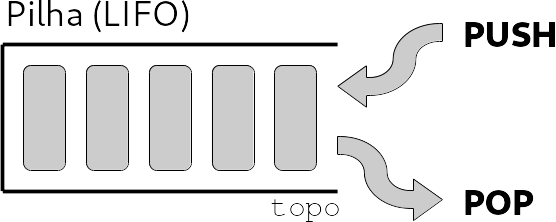
\includegraphics[height=0.3\paperheight]{imagens/pilha.png}
\end{figure}
\end{itemize}
\end{frame}

%-------------------------------------------------------
\begin{frame}\frametitle{Pilha: Implementações Possíveis}
\begin{itemize}
	\item \textbf{Arranjo}
\begin{figure}[h]
	\flushleft
	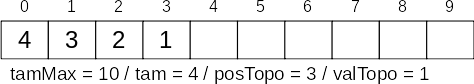
\includegraphics[height=0.15\paperheight]{imagens/pilha1.png}
\end{figure}
	\item \textbf{Lista Simplesmente Encadeada}
\begin{figure}[h]
	\flushleft
	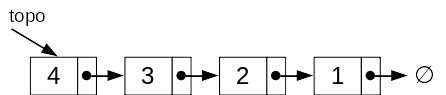
\includegraphics[height=0.15\paperheight]{imagens/pilha2.png}
\end{figure}
	\item \textbf{Lista Duplamente Encadeada}
\begin{figure}[h]
	\flushleft
	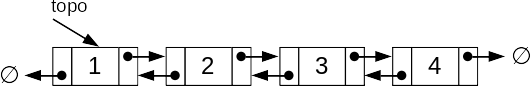
\includegraphics[height=0.15\paperheight]{imagens/pilha3.png}
\end{figure}
\end{itemize}
\end{frame}

%-------------------------------------------------------
\begin{frame}\frametitle{Aplicações que Usam Pilha}
\begin{itemize}
	\item Operações de edição de desfazer/refazer
	\item Histórico de visitação de páginas em navegadores \emph{web} (botão \emph{back})
	\item Cadeia de chamada de métodos em interpretadores e máquinas virtuais
	\item Auxiliar para implementação de outras estruturas de dados e algoritmos
	\item Implementação de compiladores
	\item Computação Gráfica (operações com matrizes)
	\item Manipulação de expressões aritméticas: infixada, pós-fixada, pré-fixada % https://ww2.inf.ufg.br/~hebert/disc/aed1/AED1_09_Pilas.pdf
\end{itemize}
\end{frame}

%-------------------------------------------------------
\begin{frame}\frametitle{Métodos do TAD Pilha}
\begin{itemize}
	\item \texttt{bool push(e)}: insere o elemento no topo da pilha (retorna \texttt{true}, em caso de sucesso, ou \texttt{false}, se NÃO houver espaço)
	\item \texttt{bool pop(\&e)}: remove e retorna (por referência) o elemento do topo da pilha (retorna \texttt{true}, em caso de sucesso, ou \texttt{false}, a pilha estiver vazia)
	\item \texttt{bool top(\&e)} ou \texttt{bool peek(\&e)}: retorna (por referência) o elemento do topo da pilha, mas não o remove da pilha (retorna \texttt{true}, em caso de sucesso, ou \texttt{false}, a pilha estiver vazia)
	\item \texttt{int size()}: retorna o número de elementos da pilha
	\item \texttt{int maxSize()}: retorna o número máximo de elementos suportado pela pilha
	\item \texttt{bool isEmpty()}: retorna \texttt{true}, se a pilha estiver vazia, ou \texttt{false}, em caso contrário
	\item \texttt{bool isFull()}: retorna \texttt{true}, se a pilha estiver cheia, ou \texttt{false}, em caso contrário
	\item \texttt{void clear()}: esvazia a pilha
\end{itemize}
\end{frame}

%-------------------------------------------------------
\begin{frame}\frametitle{Exemplo de Implementação: \texttt{IntStack.hpp}}
\lstinputlisting[basicstyle=\ttfamily\tiny]{src/IntStack.hpp}
\end{frame}

%-------------------------------------------------------
\begin{frame}\frametitle{Exemplo de Implementação: \texttt{IntStack.cpp}}
\fontsize{3pt}{5pt}\selectfont{
\lstinputlisting{src/IntStack.cpp}
}
\end{frame}
	
%-------------------------------------------------------
\begin{frame}\frametitle{Exemplo de Implementação: \texttt{IntStackMain.cpp}}
\fontsize{5pt}{6pt}\selectfont{
\lstinputlisting{src/IntStackMain.cpp}
}
\end{frame}
%-------------------------------------------------------
\begin{frame}\frametitle{Exemplo de Implementação (Saída)}
\lstinputlisting[basicstyle=\ttfamily\scriptsize]{src/IntStackApp.output}
\end{frame}

%=======================================================
\section{Exercícios}

%-------------------------------------------------------
\begin{frame}[fragile]\frametitle{Exercícios}
\begin{enumerate}
{\small
	\item Considerando como base a implementação da classe \texttt{IntStack} (apresentadas nas lâminas anteriores), implemente uma classe em C++ para gerenciar uma pilha de caracteres (\texttt{CharStack}).
	\item Usando a classe da questão anterior, escreva um programa em C++, que inverte as letras de cada palavra de um texto terminado por ponto (.) preservando a ordem das palavras.\\
Por exemplo, dado o texto:\\
\begin{verbatim}
ESTE EXERCICIO E MUITO FACIL.
\end{verbatim}
A saída deve ser:
\begin{verbatim}
ETSE OICICREXE E OTIUM LICAF
\end{verbatim}
\item Considerando ainda a classe \texttt{CharStack}, escreva uma função que verifique se uma palavra (\texttt{string}) é um palíndromo.
\item Implemente uma função em C++ para testar se duas pilhas de caracteres (objetos da classe \texttt{CharStack}), \texttt{P1} e \texttt{P2}, são iguais.
\item Implemente uma função em C++ para copiar os elementos de uma pilha Desenvolva uma operação para copiar elementos de uma pilha \texttt{P1} para uma pilha \texttt{P2} (sem destruir \texttt{P1}).
}
\end{enumerate}
\end{frame}

%=======================================================
\section{Implementando uma Pilha Encadeada}

%-------------------------------------------------------
\begin{frame}\frametitle{Estruturas Lineares Encadeadas}
\begin{itemize}
	\item Uma estrutura encadeada é uma estrutura composta por nodos, que possuem campos que apontam para outros nodos
	\item Por exemplo, em uma lista simplesmente encadeada, tipicamente:
	\begin{itemize}
		\item Há um ponteiro para o primeiro elemento da lista
		\item Cada nodo tem um campo que aponta para o próximo elemento da lista
		\item O campo de encadeamento do último elemento contém uma referência inválida
	\end{itemize}
\begin{figure}[h]
	\centering
	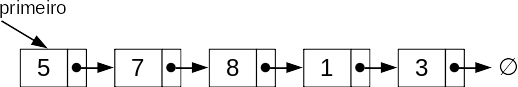
\includegraphics[height=0.15\paperheight]{imagens/lista_simplesmente_encadeada2.png}
\end{figure}
	\item Ao inserir um elemento, deve-se alocar um nodo, preenchê-lo e colocá-lo na posição desejada na estrutura (ajustando as referências necessárias)
	\item Ao remover um elemento, é preciso removê-lo (ajustando as referências necessárias) e desalocá-lo
\end{itemize}
\end{frame}

%-------------------------------------------------------
\begin{frame}[fragile]\frametitle{Estruturas Encadeadas em C++}
\begin{itemize}
	\item Pode-se declarar um nodo em C++, para armazenar caracteres, da seguinte forma:
\begin{lstlisting}[basicstyle=\ttfamily\scriptsize]
struct Nodo {
  char letra;
  Nodo *prox;
  Nodo(char l) {
    letra = l;
    next = nullptr;
  }
};
\end{lstlisting}
	\item \texttt{nullptr} é usado para indicar uma estrutura vazia ou fim da estrutura
	\item Exemplo: construção da seguinte pilha simplesmente encadeada
\begin{figure}[h]
	\centering
	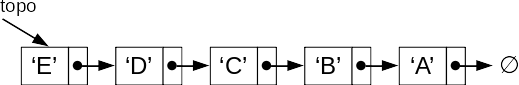
\includegraphics[height=0.15\paperheight]{imagens/pilha_simplesmente_encadeada.png}
\end{figure}
\end{itemize}
\end{frame}

%-------------------------------------------------------
\begin{frame}[fragile]\frametitle{Exemplo: \texttt{pilha\_simplesmente\_encadeada.cpp}}
\fontsize{5pt}{5pt}\selectfont{
\lstinputlisting{src/pilha_simplesmente_encadeada.cpp}
}
\end{frame}

%-------------------------------------------------------
\begin{frame}[fragile]\frametitle{Exercícios 6 e 7}
\begin{enumerate}
        \setcounter{enumi}{5}
	\item Modifique o programa da lâmina anterior para que a lista seja criada \textbf{com um laço}, exatamente com o mesmo conteúdo e na mesma ordem lógica. Faça as inserções sempre pela mesma extremidade da estrutura encadeada.
	\item Usando como modelo o programa da lâmina anterior, construa em C++ a seguinte lista duplamente encadeada. Percorra a lista, mostrando o conteúdo de seus nodos, tanto do início para o fim, quanto do fim para o início.	
\begin{figure}[h]
	\centering
	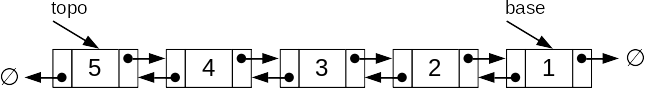
\includegraphics[height=0.16\paperheight]{imagens/pilha_duplamente_encadeada.png}
\end{figure}
\end{enumerate}
\end{frame}

%-------------------------------------------------------
\begin{frame}[fragile]\frametitle{Exercício 8}
\begin{enumerate}
        \setcounter{enumi}{7}
	\item Usando como ponto de partida a classe \texttt{IntStack}, apresentada anteriormente e implementada usando alocação sequencial ou contígua, implemente a classe \texttt{IntLinkedStack}, que funciona da mesma forma, porém usando alocação encadeada.\\
	Observações:
	\begin{itemize}
		\item A versão usando alocação encadeada eliminará a necessidade de se trabalhar com um limite máximo de elementos, consequentemente, os métodos \texttt{maxSize()} e \texttt{isFull()} NÃO farão parte da nova implementação.
		\item A definição da classe (arquivo \texttt{IntLinkedStack.hpp}) e um programa de teste ((arquivo \texttt{IntLinkedStackMain.cpp})) estão listados nas lâminas a seguir.
	\end{itemize}
\end{enumerate}
\end{frame}

%-------------------------------------------------------
\begin{frame}[fragile]\frametitle{Exercício 8: \texttt{IntLinkedStack.hpp}}
\lstinputlisting[basicstyle=\ttfamily\tiny]{src/IntLinkedStack.hpp}
\end{frame}

%-------------------------------------------------------
\begin{frame}[fragile]\frametitle{Exercício 8: \texttt{IntLinkedStackMain.cpp}}
\fontsize{6pt}{6pt}\selectfont{
\lstinputlisting{src/IntLinkedStackMain.cpp}
}
\end{frame}

%=======================================================
\section{Fila (\emph{Queue})}

%-------------------------------------------------------
\begin{frame}\frametitle{Fila ou \emph{Queue}}
\begin{itemize}
	\item Usa a política \emph{FIFO -- First In First Out} (o primeiro que entrou, é o primeiro a sair)
	\item Possui uma entrada (fim), a partir da qual os dados são inseridos, e uma saída (início), a partir da qual os dados são removidos
\begin{figure}[h]
	\centering
	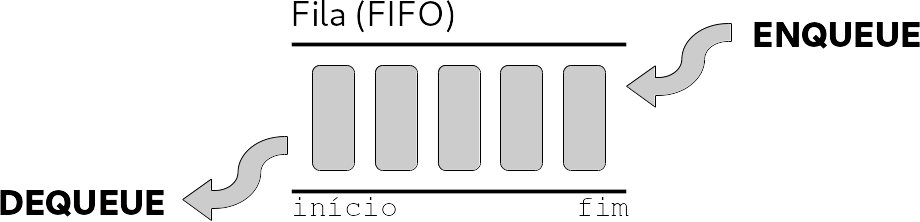
\includegraphics[height=0.3\paperheight]{imagens/fila.png}
\end{figure}
\end{itemize}
\end{frame}

%-------------------------------------------------------
\begin{frame}\frametitle{Fila: Implementações Possíveis}
\begin{itemize}
	\item \textbf{Arranjo circular}
\begin{figure}[h]
	\flushleft
	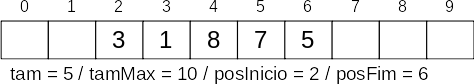
\includegraphics[height=0.13\paperheight]{imagens/fila1a.png} ~ ~ ~ 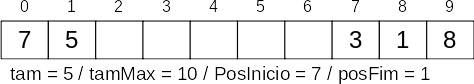
\includegraphics[height=0.13\paperheight]{imagens/fila1b.png}
\end{figure}
	\item \textbf{Lista Simplesmente Encadeada}
\begin{figure}[h]
	\flushleft
	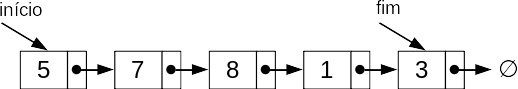
\includegraphics[height=0.15\paperheight]{imagens/fila2.png}
\end{figure}
	\item \textbf{Lista Duplamente Encadeada}
\begin{figure}[h]
	\flushleft
	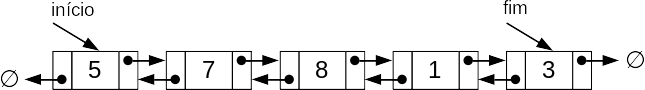
\includegraphics[height=0.15\paperheight]{imagens/fila3.png}
\end{figure}
\end{itemize}
\end{frame}

%-------------------------------------------------------
\begin{frame}[fragile]\frametitle{Implementação de um Arranjo Circular}
\begin{itemize}
	\item Usam-se índices para inserção (\texttt{insertPos}) e remoção (\texttt{removePos}) que percorrem o arranjo (\texttt{queue}) de forma ``circular''
	\item Para inserir pode-se usar:
\begin{lstlisting}[basicstyle=\ttfamily\scriptsize]
queue[ insertPos++ ] = e;
insertPos %= maxElements; // Ou: if ( insertPos == maxElements ) insertPos = 0;
\end{lstlisting}
	\item Para remover pode-se usar:
\begin{lstlisting}[basicstyle=\ttfamily\scriptsize]
e = queue[ removePos++ ];
removePos %= maxElements; // Ou: if ( removePos == maxElements ) removePos = 0;
\end{lstlisting}
	\item Deve-se verificar as situações de arranjo cheio (na inserção) e arranjo vazio (na remoção)
	\item Exemplos:
\begin{figure}[h]
	\flushleft
	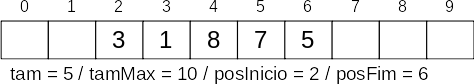
\includegraphics[height=0.13\paperheight]{imagens/fila1a.png} ~ ~ ~ 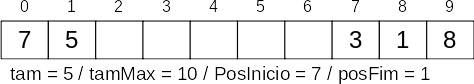
\includegraphics[height=0.13\paperheight]{imagens/fila1b.png}
\end{figure}
\end{itemize}
\end{frame}

%-------------------------------------------------------
\begin{frame}\frametitle{Aplicações que Usam Fila}
\begin{itemize}
	\item Desenvolvimento de aplicativos
	\begin{itemize}
		\item Gerenciamento de transações para aplicativos de lojas, teatros, centros de reserva, etc.
	\end{itemize}
	\item Simulações
	\begin{itemize}
		\item Listas de espera na simulação de sistemas de atendimento (banco, supermercado, etc.)
	\end{itemize}
	\item Sistemas Operacionais
	\begin{itemize}
		\item Fila de documentos para impressão
		\item Escalonamento de processos em um sistema operacional
		\item Fila de requisições de acesso a disco
		\item Fila de espera por recursos
		\item Fila (\emph{buffering}) de mensagens e pacotes
	\end{itemize}
	\item Estruturas de Dados
	\begin{itemize}
		\item Suporte na implementação de algoritmos sobre árvores e grafos
	\end{itemize}
	\item etc.
\end{itemize}
\end{frame}

%-------------------------------------------------------
\begin{frame}\frametitle{Métodos do TAD Fila (\emph{Queue})}
\begin{itemize}
	\item \texttt{bool enqueue(e)}: insere o elemento no final da fila (retorna \texttt{true}, em caso de sucesso, ou \texttt{false}, se NÃO houver espaço)
	\item \texttt{bool dequeue(\&e)}: remove e retorna (por referência) o elemento do início da fila (retorna \texttt{true}, em caso de sucesso, ou \texttt{false}, a fila estiver vazia)
	\item \texttt{bool head(\&e)}: retorna (por referência) o elemento do início da fila, mas não o remove da fila (retorna \texttt{true}, em caso de sucesso, ou \texttt{false}, a fila estiver vazia)
	\item \texttt{int size()}: retorna o número de elementos da fila
	\item \texttt{int maxSize()}: retorna o número máximo de elementos suportado pela fila
	\item \texttt{bool isEmpty()}: retorna \texttt{true}, se a fila estiver vazia, ou \texttt{false}, em caso contrário
	\item \texttt{bool isFull()}: retorna \texttt{true}, se a fila estiver cheia, ou \texttt{false}, em caso contrário
	\item \texttt{void clear()}: esvazia a fila
\end{itemize}
\end{frame}

%-------------------------------------------------------
\begin{frame}\frametitle{Exemplo de Implementação: \texttt{IntQueue.hpp}}
\lstinputlisting[basicstyle=\ttfamily\tiny]{src/IntQueue.hpp}
\end{frame}

%-------------------------------------------------------
\begin{frame}\frametitle{Exemplo de Implementação: \texttt{IntQueue.cpp}}
\fontsize{3pt}{5pt}\selectfont{
\lstinputlisting{src/IntQueue.cpp}
}
\end{frame}
	
%-------------------------------------------------------
\begin{frame}\frametitle{Exemplo de Implementação: \texttt{IntQueueMain.cpp}}
\fontsize{5pt}{6pt}\selectfont{
\lstinputlisting{src/IntQueueMain.cpp}
}
\end{frame}
%-------------------------------------------------------
\begin{frame}\frametitle{Exemplo de Implementação (Saída)}
\lstinputlisting[basicstyle=\ttfamily\scriptsize]{src/IntQueueApp.output}
\end{frame}

%-------------------------------------------------------
\begin{frame}[fragile]\frametitle{Exercício 9}
\begin{enumerate}
        \setcounter{enumi}{8}
	\item Considere duas estrutura de dados do tipo fila, chamadas \texttt{A} e \texttt{B}. Na fila \texttt{A}, foram inseridos (nessa ordem) os seguintes valores: 10, 20 e 30. E, na fila \texttt{B}, foram inseridos (nessa ordem) os seguintes valores: 30, 20 e 10. Para ambas as estruturas, considere as seguintes operações:
\begin{itemize}
	\item \texttt{dequeue(F)}: que remove um elemento da fila \texttt{F} e retorna esse elemento;
	\item \texttt{enqueue(F, E)}: que insere o elemento \texttt{E} na fila \texttt{F};
	\item \texttt{head(F)}: que retorna o elemento do início da fila, sem removê-lo da estrutura.
\end{itemize}
Quais serão as sequências de elementos nas filas \texttt{A} e \texttt{B}, após executar a expressão ``\texttt{enqueue(A, dequeue(A) + dequeue(B) + head(A))}''?
\end{enumerate}
\end{frame}

%-------------------------------------------------------
\begin{frame}[fragile]\frametitle{Exercício 10}
\begin{enumerate}
        \setcounter{enumi}{9}
	\item Usando como ponto de partida a classe \texttt{IntQueue}, apresentada anteriormente e implementada usando alocação sequencial ou contígua, implemente a classe \texttt{IntLinkedQueue}, que funciona da mesma forma, porém usando alocação encadeada.\\
	Observações:
	\begin{itemize}
		\item A versão usando alocação encadeada eliminará a necessidade de se trabalhar com um limite máximo de elementos, consequentemente, os métodos \texttt{maxSize()} e \texttt{isFull()} NÃO farão parte da nova implementação.
		\item A definição da classe (arquivo \texttt{IntLinkedQueue.hpp}) e um programa de teste ((arquivo \texttt{IntLinkedQueueMain.cpp})) estão listados nas lâminas a seguir.
	\end{itemize}
\end{enumerate}
\end{frame}

%-------------------------------------------------------
\begin{frame}[fragile]\frametitle{Exercício 10: \texttt{IntLinkedQueue.hpp}}
\lstinputlisting[basicstyle=\ttfamily\tiny]{src/IntLinkedQueue.hpp}
\end{frame}

%-------------------------------------------------------
\begin{frame}[fragile]\frametitle{Exercício 10: \texttt{IntLinkedQueueMain.cpp}}
\fontsize{6pt}{6pt}\selectfont{
\lstinputlisting{src/IntLinkedQueueMain.cpp}
}
\end{frame}

%=======================================================
\section{Créditos}

%-------------------------------------------------------
\begin{frame}\frametitle{Créditos}
\begin{itemize}
	\item Estas lâminas contêm trechos inspirados em materiais criados e disponibilizados pelos professores Isabel Harb Manssour e Iaçanã Ianiski Weber.
\end{itemize}
\end{frame}

%=======================================================
\section{Soluções}

%-------------------------------------------------------
\begin{frame}[fragile]\frametitle{Exercício 1: \texttt{CharStack.hpp}}
\lstinputlisting[basicstyle=\ttfamily\tiny]{src/CharStack.hpp}
\end{frame}

%-------------------------------------------------------
\begin{frame}[fragile]\frametitle{Exercício 1: \texttt{CharStack.cpp}}
\fontsize{5pt}{5pt}\selectfont{
\lstinputlisting{src/CharStack.cpp}
}
\end{frame}

%-------------------------------------------------------
\begin{frame}[fragile]\frametitle{Exercício 2: \texttt{questao2.cpp}}
\lstinputlisting[basicstyle=\ttfamily\tiny]{src/questao2.cpp}
\end{frame}

%-------------------------------------------------------
\begin{frame}[fragile]\frametitle{Exercício 6: \texttt{pilha\_simplesmente\_encadeada2.cpp}}
\fontsize{6pt}{6pt}\selectfont{
\lstinputlisting{src/pilha_simplesmente_encadeada2.cpp}
}
\end{frame}

%-------------------------------------------------------
\begin{frame}[fragile]\frametitle{Exercício 7: \texttt{pilha\_duplamente\_encadeada.cpp}}
\fontsize{5pt}{5pt}\selectfont{
\lstinputlisting{src/pilha_duplamente_encadeada.cpp}
}
\end{frame}

%-------------------------------------------------------
\begin{frame}[fragile]\frametitle{Exercício 8: \texttt{IntLinkedStack.cpp}}
\fontsize{3pt}{5pt}\selectfont{
\lstinputlisting{src/IntLinkedStack.cpp}
}
\end{frame}

%-------------------------------------------------------
\begin{frame}[fragile]\frametitle{Exercício 9}
\begin{verbatim}
A = { 20, 30, 60 }
B = { 20, 10 }
\end{verbatim}
\end{frame}

%-------------------------------------------------------
\begin{frame}[fragile]\frametitle{Exercício 8: \texttt{IntLinkedQueue.cpp}}
\fontsize{3pt}{5pt}\selectfont{
\lstinputlisting{src/IntLinkedQueue.cpp}
}
\end{frame}

%-------------------------------------------------------
\end{document}

